\chapter{Digital Twin and Machine Learning Layer}

\section{Introduction}

This chapter presents the Digital Twin and machine learning layer of Agrio. It explains how timestamped sensor and environmental records are prepared for Random Forest training, how the exported models are used by the ML service, how prediction outputs update the Digital Twin state, and how simulation and recommendation functions support irrigation decisions.

\section{Virtual zone state}

The zone state is the central representation of the Digital Twin. It stores current moisture, soil temperature, water balance, stress level, irrigation need, recommended action, pump status, synchronization information, prediction confidence, and timestamps. This state is updated whenever new sensor data arrives or when prediction and simulation processes run.

\section{Dataset adaptation and feature engineering}

The machine-learning layer requires a structured tabular dataset before model training. In Agrio, the objective of the dataset-preparation stage is to transform timestamped irrigation and environmental records into numerical features that can be used by Random Forest models. The preparation workflow includes cleaning, normalization, feature engineering, target separation, model training, evaluation, and metadata export.

Figure~\ref{fig:dataset_feature_engineering_workflow} presents this preparation workflow in a simplified form. The figure focuses on the implemented dataset transformation process and intentionally avoids unsupported elements such as online learning, crop-growth modelling, yield prediction, or complex optimization. The goal is to show how the dataset becomes suitable for two prediction tasks: estimating irrigation need and suggesting an irrigation hour.

\begin{figure}[H]
    \centering
    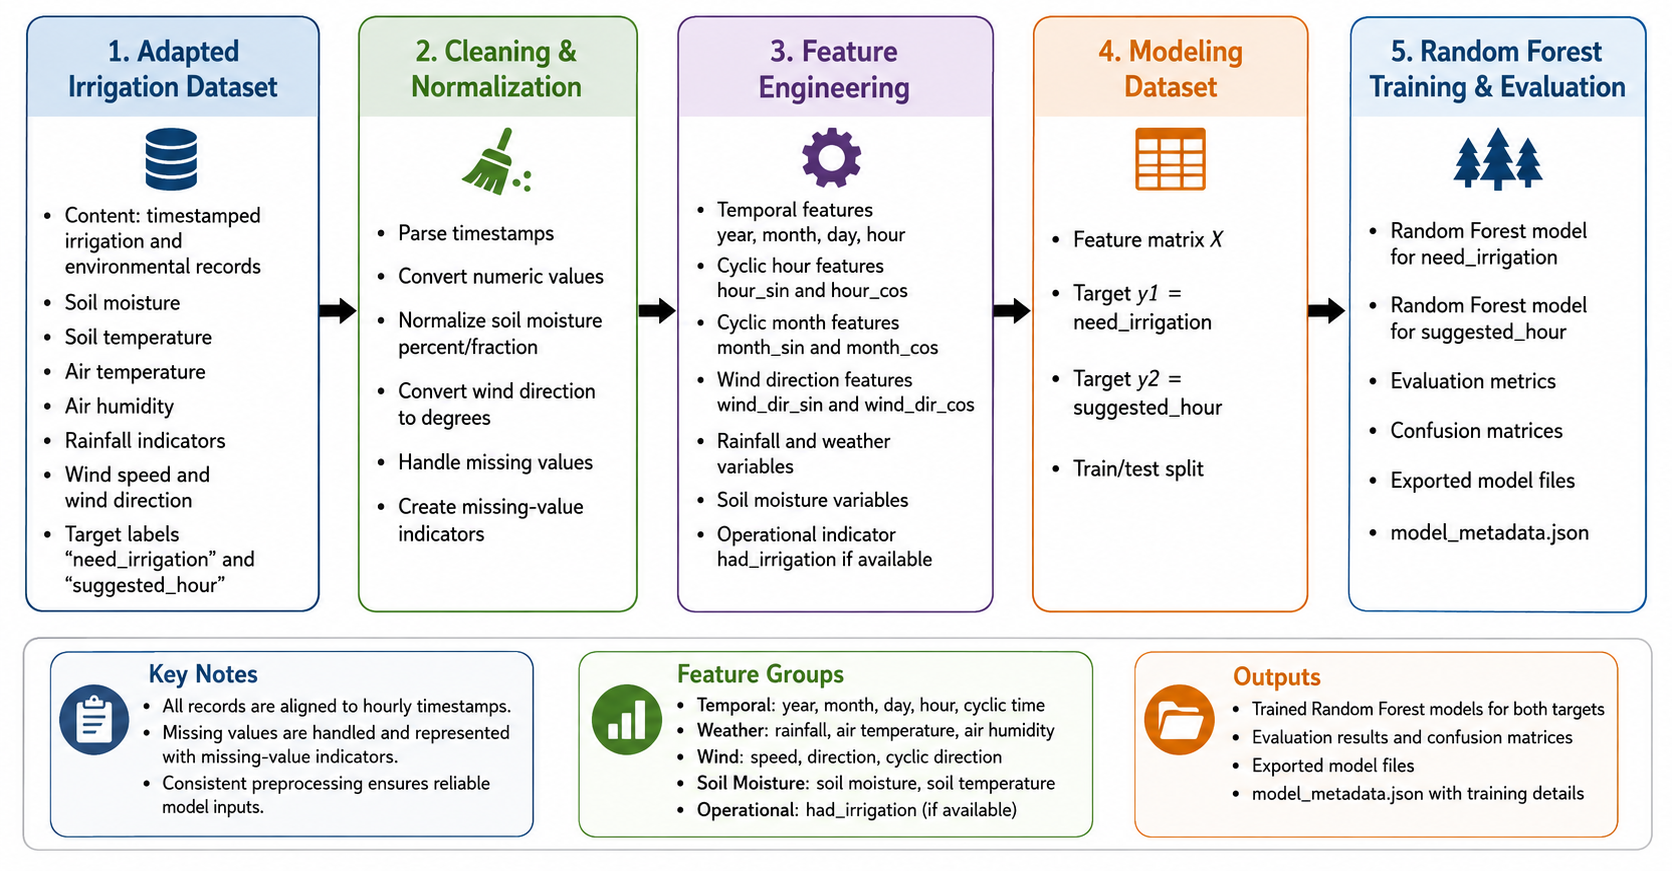
\includegraphics[width=0.95\textwidth]{figures/chapter_08/figure_8_1_dataset_adaptation_clean.png}
    \caption{Dataset adaptation and feature engineering workflow used before Random Forest training.}
    \label{fig:dataset_feature_engineering_workflow}
\end{figure}

Figure~\ref{fig:dataset_feature_engineering_workflow} is read from left to right. The first stage is the adapted irrigation dataset. The input records contain timestamped measurements and weather-style variables, including soil moisture, air temperature, air humidity, rainfall indicators, wind speed, and wind direction. The dataset also contains target labels used for supervised learning: \texttt{need\_irrigation} and \texttt{suggested\_hour}.

The second stage is cleaning and normalization. Timestamps are parsed into structured temporal information, numeric values are converted to consistent formats, soil moisture values are normalized between fraction and percentage representations, and wind direction is converted from categorical compass notation into numerical degrees when necessary. Missing values are handled explicitly, and missing-value indicators are created for variables that may be absent from some records.

The third stage is feature engineering. Temporal features such as year, month, day, and hour are extracted from timestamps. Cyclic features are created for hour and month using sine and cosine transformations. Wind direction is also encoded using sine and cosine components. These cyclic encodings are useful because they preserve the circular nature of time and direction: for example, hour 23 and hour 0 are close in time even though their numeric values appear far apart.

The fourth stage is the construction of the modeling dataset. The feature matrix \texttt{X} is separated from the target variables. The first target, \texttt{need\_irrigation}, corresponds to the binary irrigation-decision task. The second target, \texttt{suggested\_hour}, corresponds to the irrigation-hour prediction task. The dataset is then split into training and testing subsets for evaluation.

The fifth stage is Random Forest training and evaluation. One Random Forest model is trained to predict whether irrigation is needed, while a second Random Forest model is trained to predict the suggested irrigation hour. The trained models and their metadata are exported so that the ML service can load them during inference. The exported metadata also documents the feature list, target variables, model paths, and evaluation metrics.

These results should be interpreted as machine-learning evaluation results on the prepared dataset. They do not replace agronomic field validation over a complete growing season. Instead, they validate that the ML pipeline can transform input features into reproducible prediction outputs used by the Digital Twin and recommendation workflow.

\begin{table}[H]
\centering
\small
\setlength{\tabcolsep}{3pt}
\caption{Main feature groups used by the Random Forest models.}
\label{tab:ml_feature_groups}
\begin{tabular}{p{0.26\textwidth}p{0.62\textwidth}}
\hline
\textbf{Feature group} & \textbf{Examples} \\
\hline
Temporal features & \texttt{year}, \texttt{month}, \texttt{day}, \texttt{hour}. \\
Cyclic time features & \texttt{hour\_sin}, \texttt{hour\_cos}, \texttt{month\_sin}, \texttt{month\_cos}. \\
Weather features & \texttt{air\_temperature\_c}, \texttt{air\_humidity\_pct}, \texttt{precipitation\_mm}, \texttt{rainfall\_hour\_mm}, \texttt{rainfall\_day\_mm}. \\
Wind features & \texttt{wind\_speed\_kmh}, \texttt{wind\_direction\_deg}, \texttt{wind\_dir\_sin}, \texttt{wind\_dir\_cos}. \\
Soil moisture features & \texttt{soil\_moisture\_pct}, \texttt{soil\_moisture\_fraction}. \\
Operational and missing-value indicators & \texttt{had\_irrigation}, \texttt{soil\_temperature\_c\_missing}, \texttt{leaf\_wetness\_missing},\newline \texttt{light\_intensity\_lux\_missing}, \texttt{pressure\_missing}, \texttt{rainfall\_current\_mm\_missing}. \\
Additional suggested-hour inputs & \texttt{need\_irrigation}, \texttt{is\_favorable}. \\
\hline
\end{tabular}
\end{table}

It is important to distinguish the training workflow from the runtime inference workflow. Figure~\ref{fig:dataset_feature_engineering_workflow} describes how the dataset is prepared before model training. At runtime, the backend prepares a feature payload from the current Digital Twin state and recent measurements, sends it to the ML service, and receives prediction outputs. Therefore, the same feature logic supports both training-time reproducibility and runtime inference consistency.

\section{Random Forest model training}

The first model predicts \texttt{need\_irrigation}. This is a binary classification task where the output indicates whether irrigation is required under the current conditions.

The second model predicts \texttt{suggested\_hour}. This task estimates the most appropriate irrigation hour based on the feature set and the irrigation-need context. The second task is treated by the exported Random Forest model as implemented in the ML service metadata.

\begin{figure}[H]
    \centering
    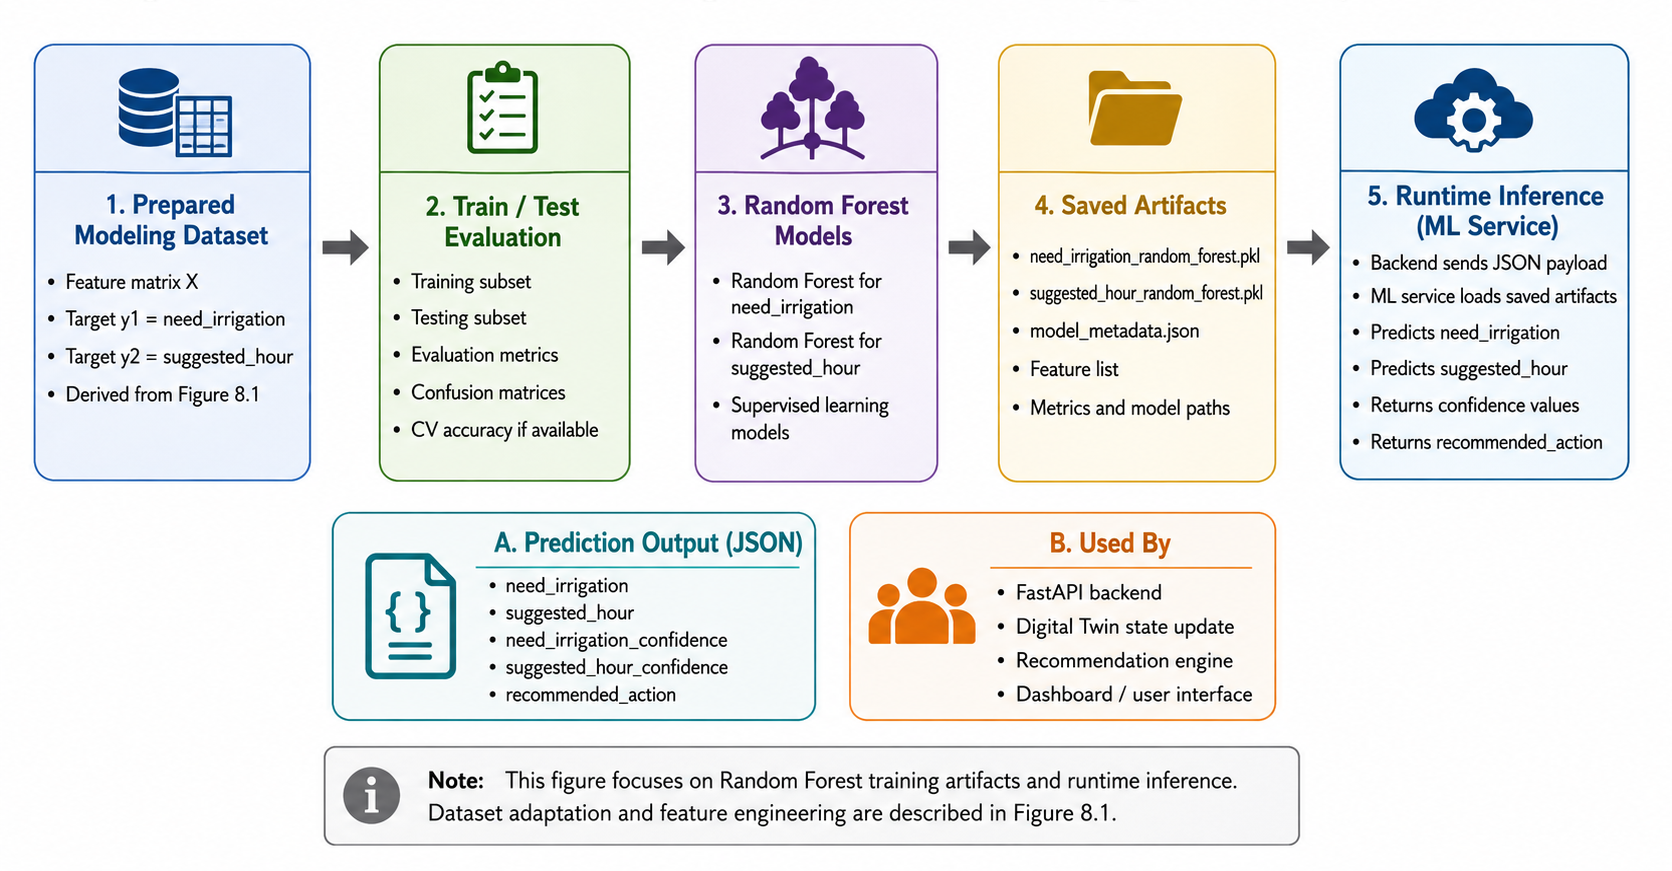
\includegraphics[width=0.9\textwidth,height=0.75\textheight,keepaspectratio]{figures/chapter_08/figure_8_2_ml_pipeline_clean.png}
    \caption{Random Forest training and runtime inference pipeline used by the ML service.}
    \label{fig:8-1-machine-learning-pipeline-from-dataset-adaptation-to-random-forest}
\end{figure}

\section{Evaluation metrics and model metadata}

The exported metadata records the model paths, target variables, feature lists, and evaluation metrics. These metrics are useful for checking that the training pipeline is reproducible and that the exported models can be loaded by the ML service. They should be interpreted as dataset-level evaluation results, not as proof of long-term agronomic validity in real field conditions.

\begin{footnotesize}
\setlength{\tabcolsep}{2pt}
\begin{longtable}{@{}>{\raggedright\arraybackslash}p{0.21\textwidth}>{\raggedright\arraybackslash}p{0.21\textwidth}>{\raggedright\arraybackslash}p{0.21\textwidth}>{\raggedright\arraybackslash}p{0.21\textwidth}@{}}
\caption{Model performance metrics from project metadata}\\
\toprule
Model & Main task & Reported metric & Interpretation \\
\midrule
\endfirsthead
\toprule
Model & Main task & Reported metric & Interpretation \\
\midrule
\endhead
Random Forest need\_irrigation & Binary irrigation need prediction & High accuracy reported in metadata & Good dataset-level performance; field validation still required \\
Random Forest suggested\_hour & Suggested irrigation hour prediction & Moderate-to-high accuracy reported in metadata & Useful for planning support, should be validated with real schedules \\
Rule-based fallback & Fallback decision when ML is unavailable & Not an ML metric & Improves system continuity when inference is unavailable \\
\bottomrule
\end{longtable}
\end{footnotesize}

\section{ML inference service}

The ML service exposes endpoints such as \texttt{/health}, \texttt{/metadata}, and \texttt{/predict}. The backend prepares a feature payload and sends it to the ML service. The response includes irrigation need, confidence, suggested hour, suggested-hour confidence, recommended action, and the features used for prediction.

\begin{figure}[H]
    \centering
    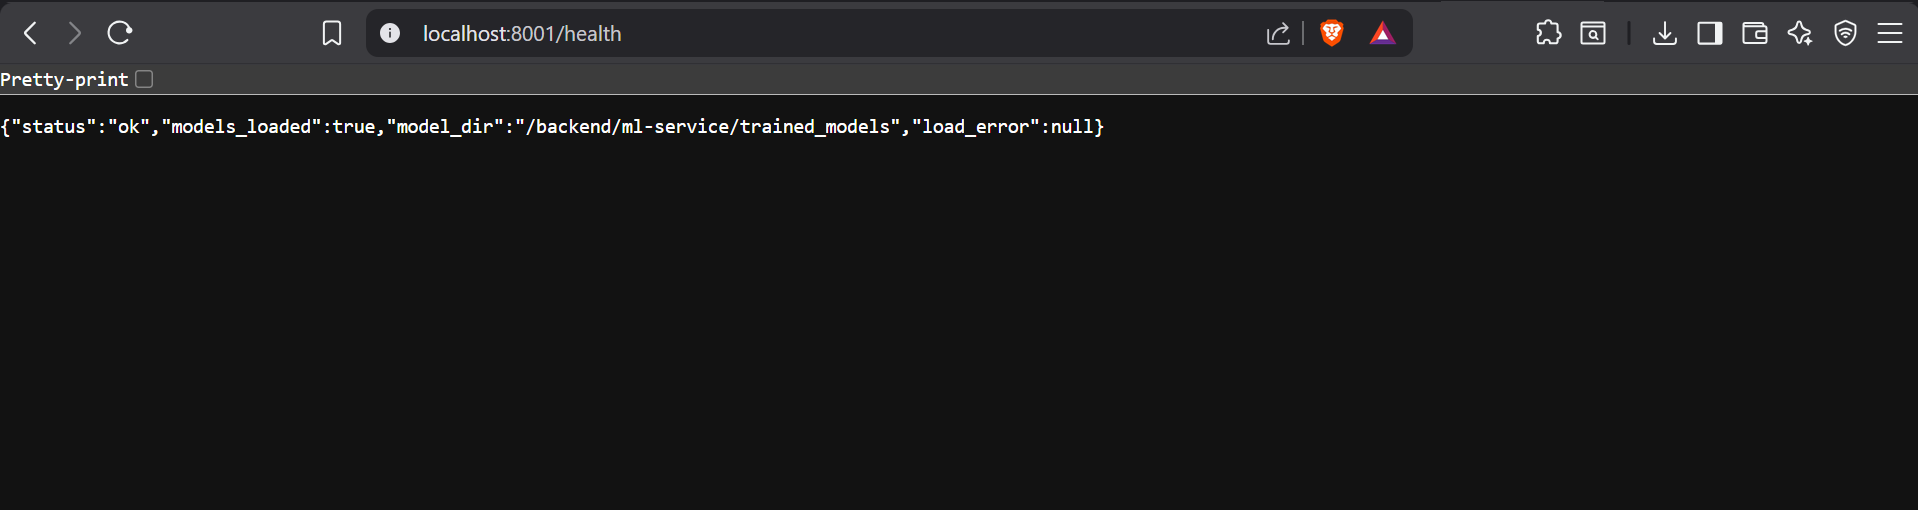
\includegraphics[width=0.9\textwidth,height=0.75\textheight,keepaspectratio]{figures/chapter_08/Figure 8.3 — ML service health endpoint showing model loading status.png}
    \caption{ML service health endpoint showing model loading status.}
    \label{fig:8-3-ml-service-health-endpoint-showing-model-loading-status}
\end{figure}

\begin{figure}[H]
    \centering
    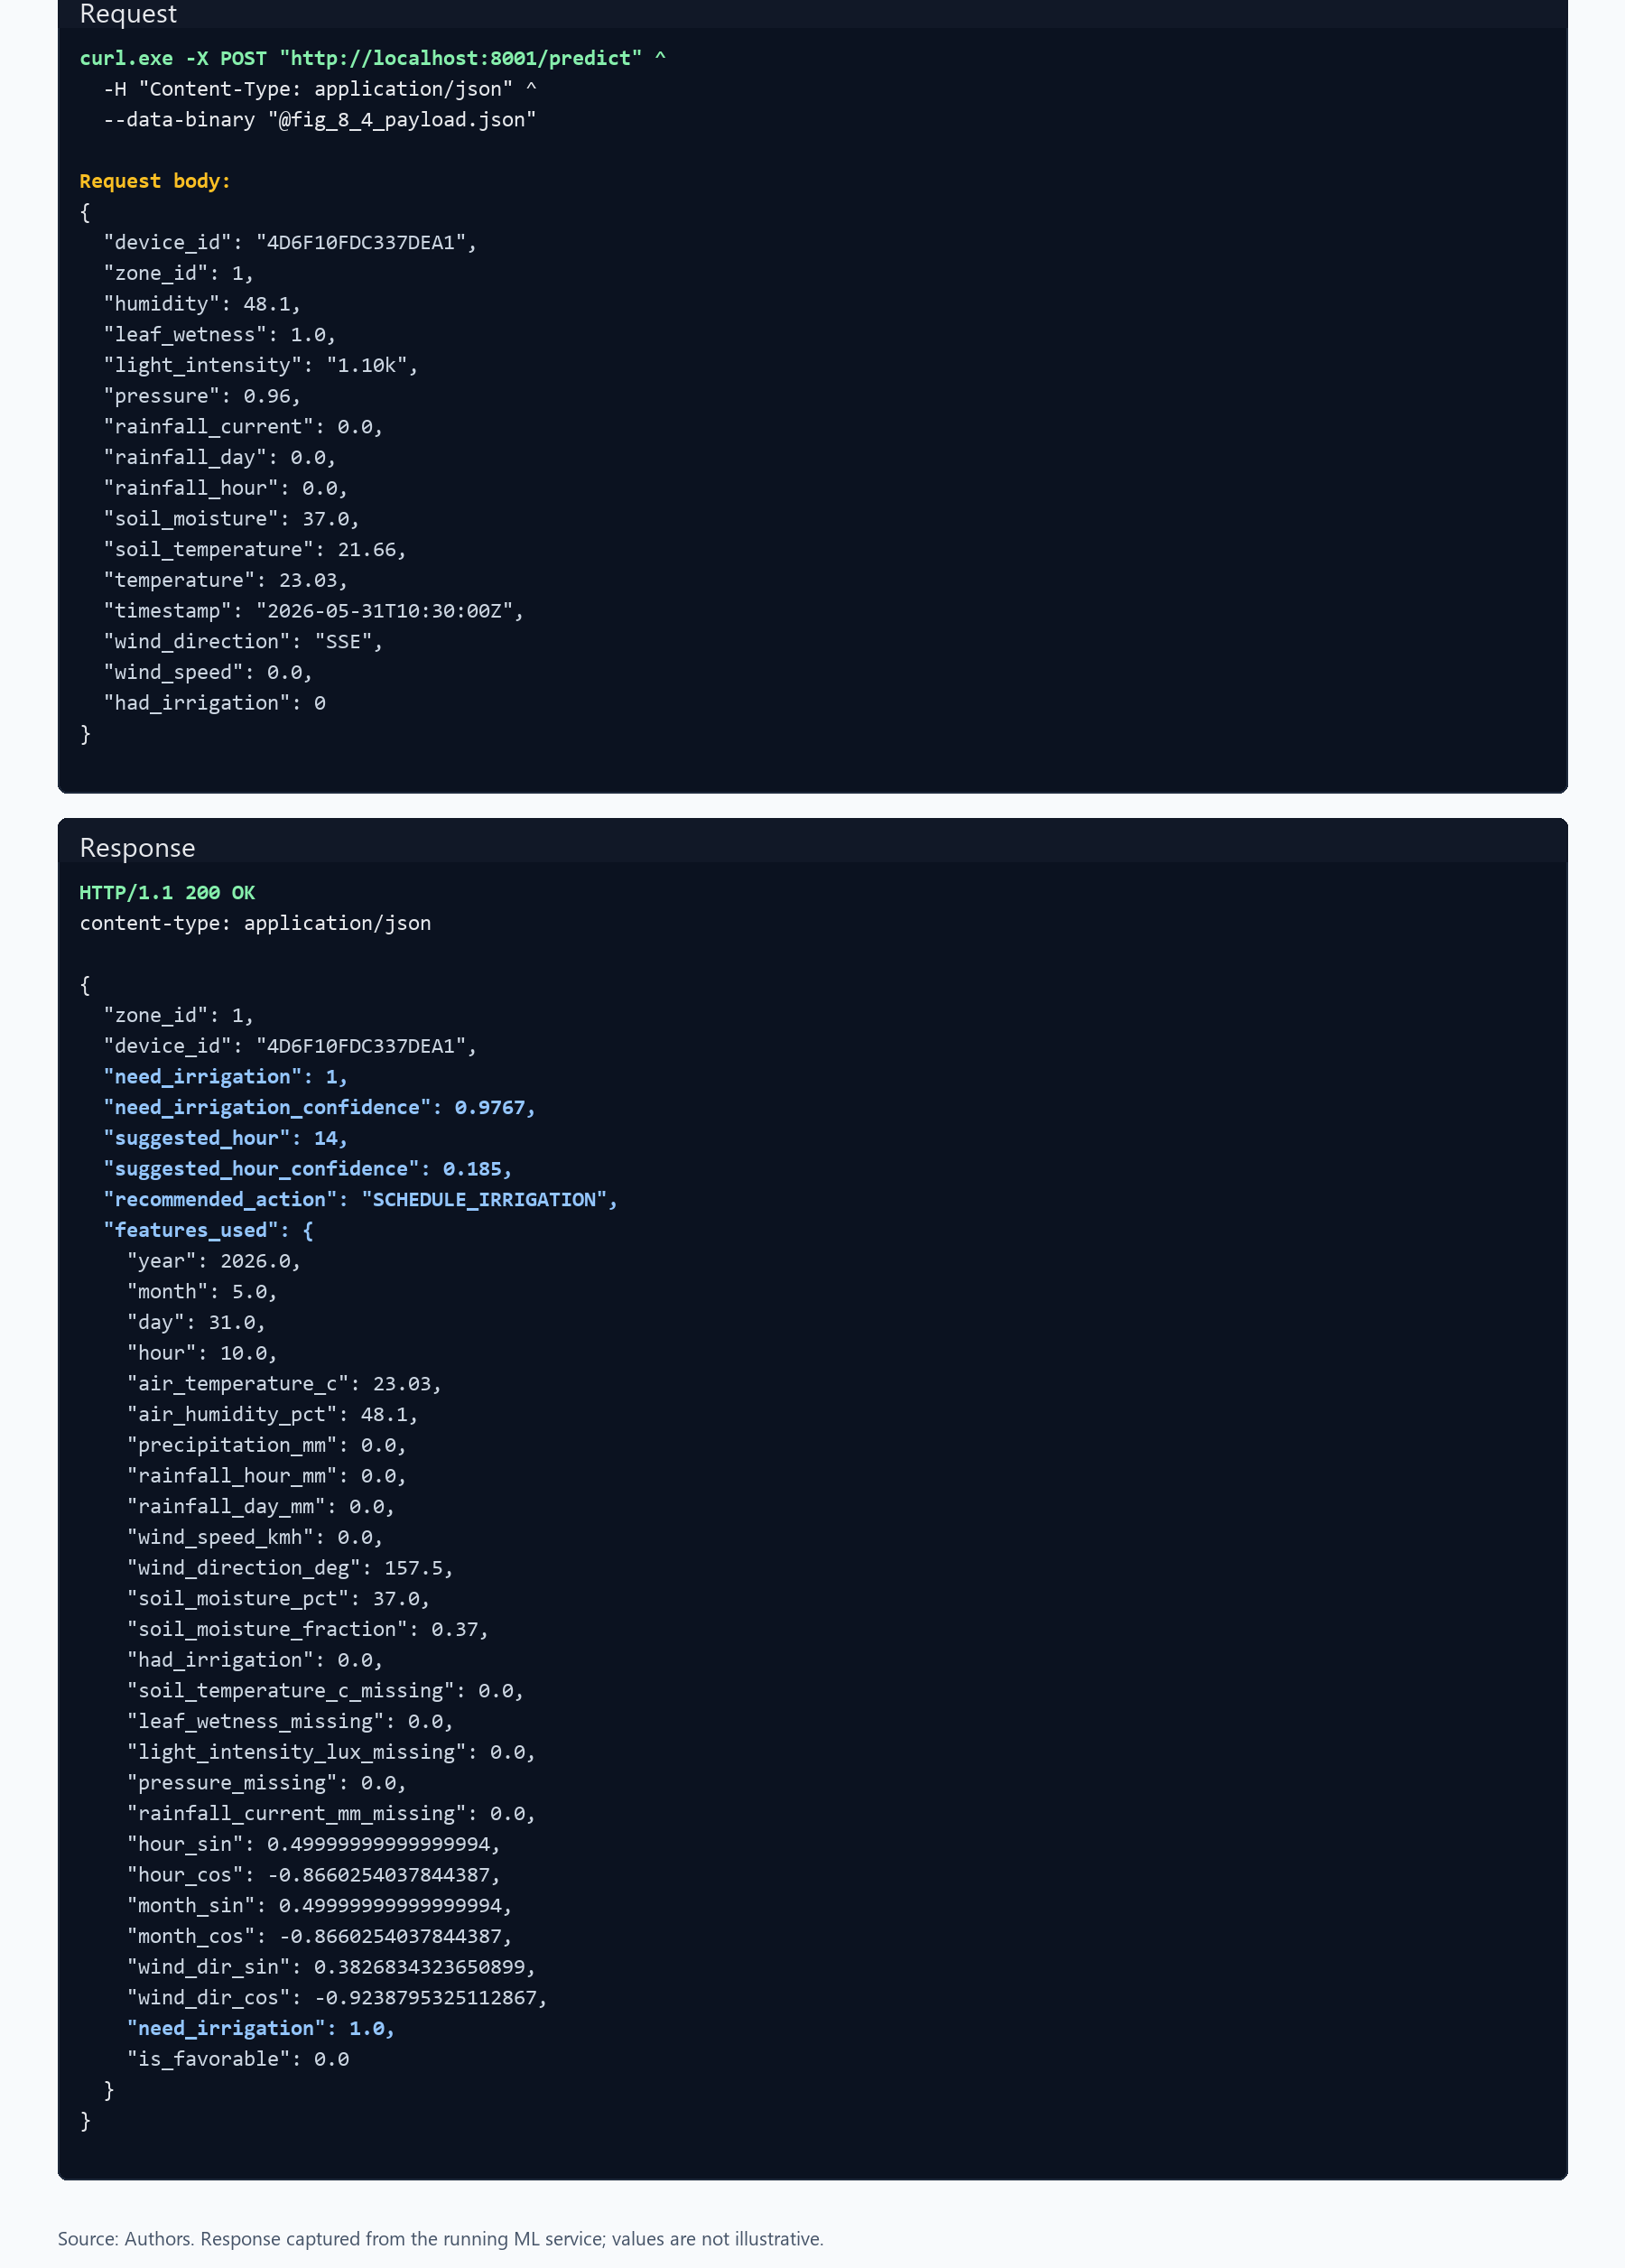
\includegraphics[width=0.9\textwidth,height=0.75\textheight,keepaspectratio]{figures/chapter_08/figure_8_4_ml_prediction_response_clean.png}
    \caption{ML prediction response for irrigation need and suggested irrigation hour.}
    \label{fig:8-4-ml-prediction-response-for-irrigation-need-and-suggested-irrigatio}
\end{figure}

\section{Digital Twin state update}

After ML inference, the backend stores prediction results and updates the zone state with AI fields. The state history table records previous states, enabling temporal analysis and validation. This creates continuity between measurements, predictions, and dashboard display.

\begin{figure}[H]
    \centering
    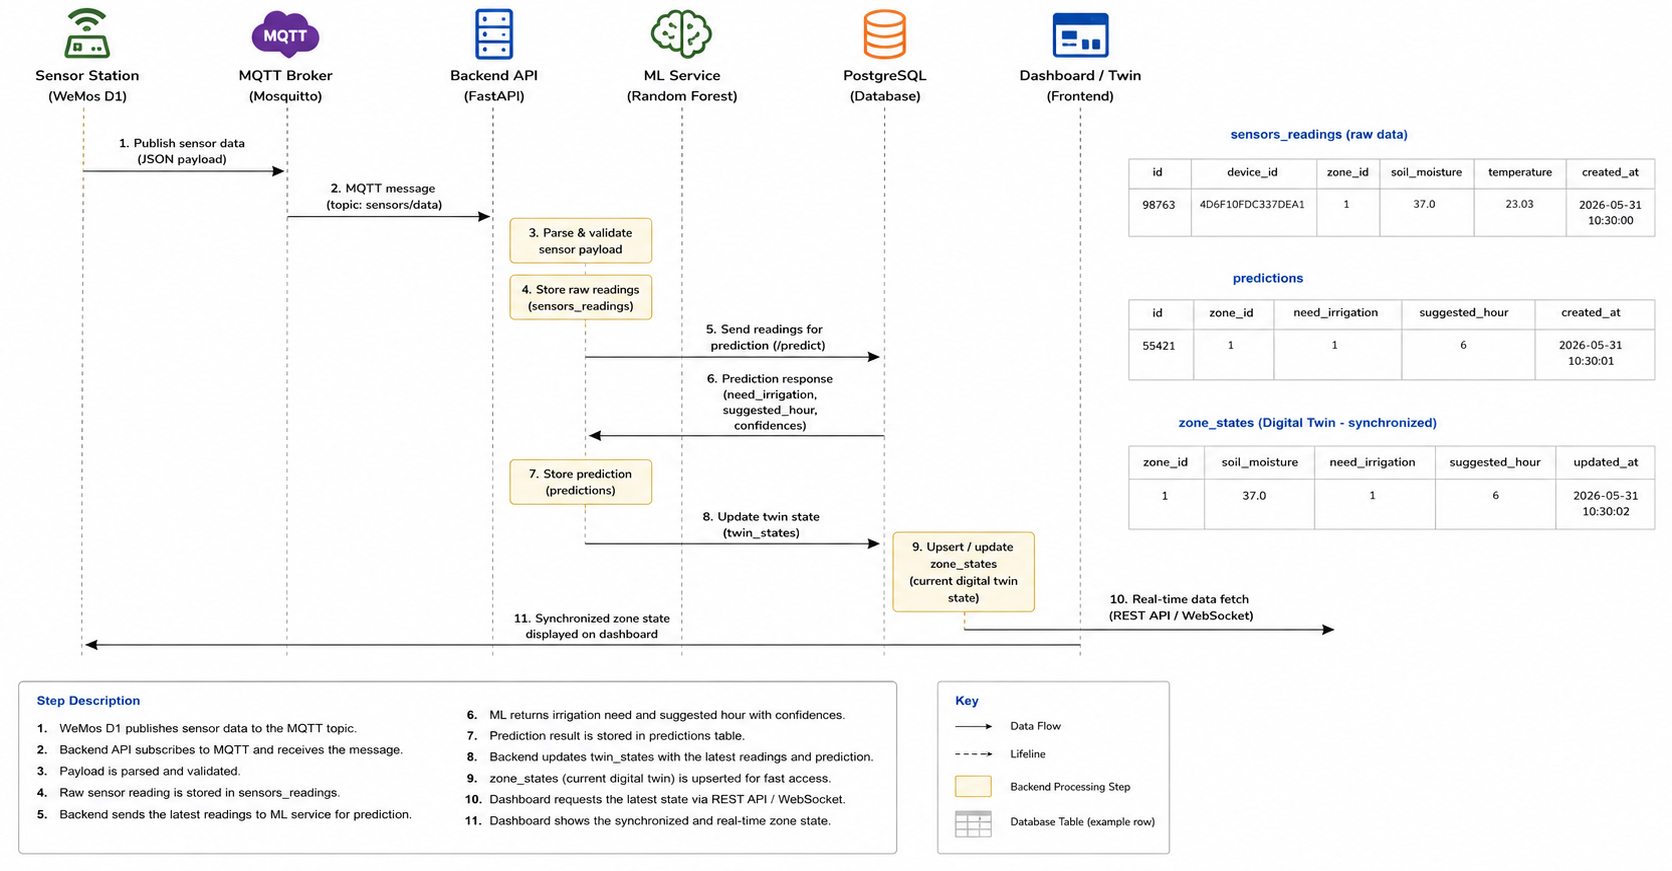
\includegraphics[width=0.9\textwidth,height=0.75\textheight,keepaspectratio]{figures/chapter_08/figure_8_5_dt_state_update_clean.png}
    \caption{Digital Twin state update flow from sensor readings to synchronized zone state.}
    \label{fig:8-5-digital-twin-state-update-flow-from-sensor-readings-to-synchronize}
\end{figure}

\section{What-if simulation and recommendation generation}

The what-if simulation compares future moisture evolution under different scenarios. Inputs include zone, irrigation duration, projection horizon, and optional flow-rate override. Outputs include simulated moisture, water balance, 24-hour and 48-hour projection, recommended action, and explanation.

\begin{figure}[H]
    \centering
    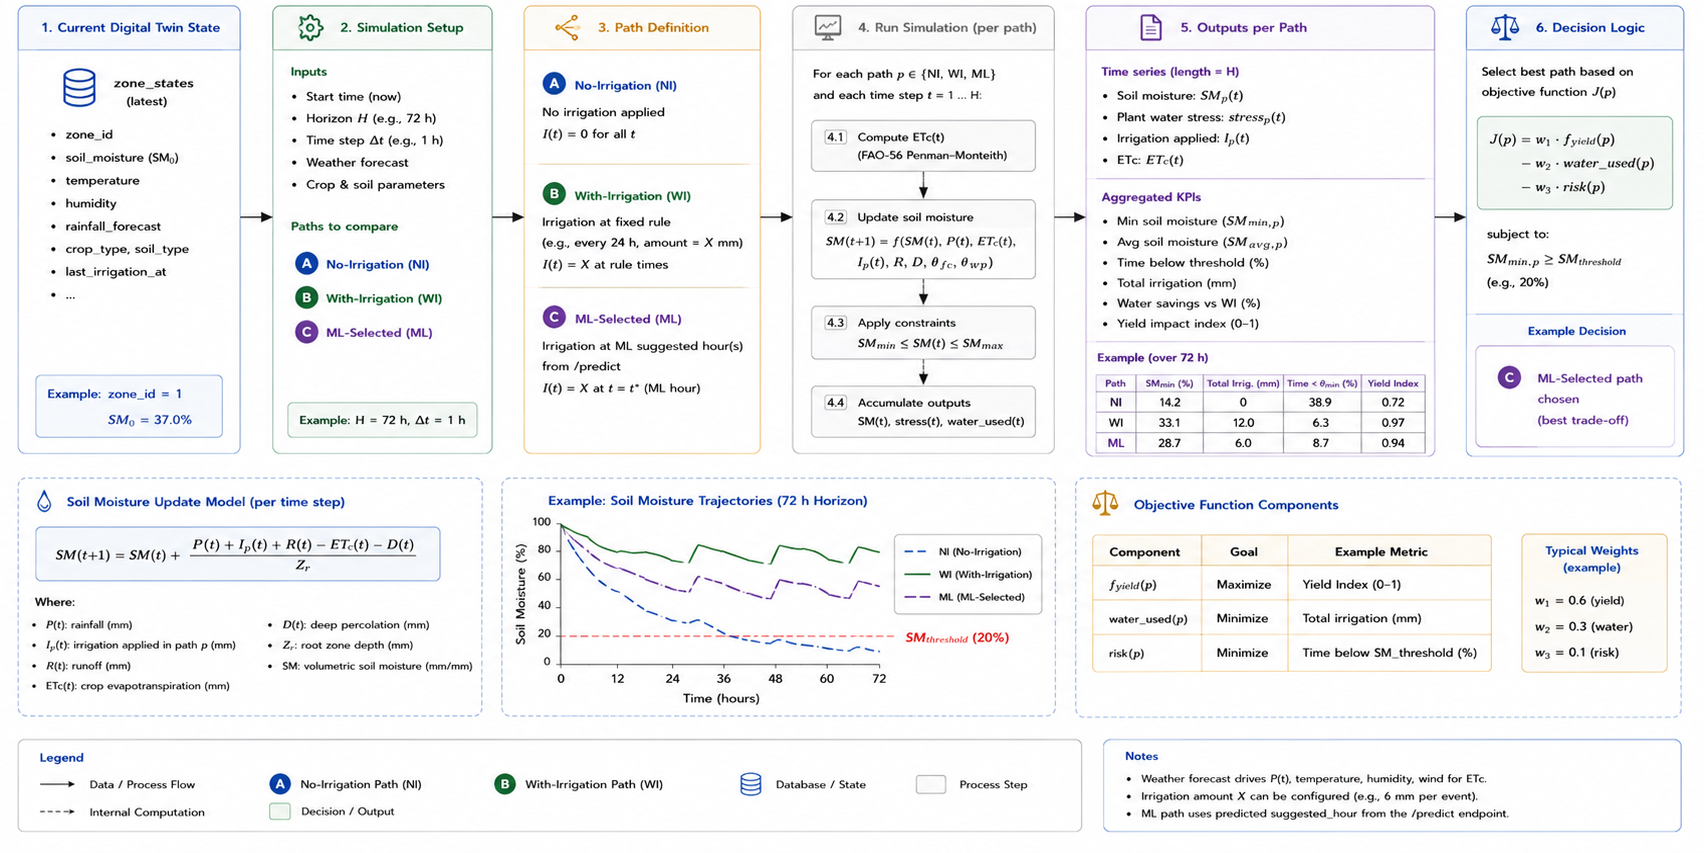
\includegraphics[width=0.9\textwidth,height=0.75\textheight,keepaspectratio]{figures/chapter_08/figure_8_6_what_if_simulation_clean.png}
    \caption{What-if simulation logic comparing no-irrigation, with-irrigation, and ML-selected paths.}
    \label{fig:8-6-what-if-simulation-logic-comparing-no-irrigation-with-irrigation-a}
\end{figure}

Recommendation generation is evaluated immediately after simulation because the recommendation engine uses the same decision context. Simulation output, current Digital Twin state, ML prediction, forecast context, and rule-based constraints are combined to decide whether the system should keep irrigation off, irrigate now, schedule irrigation for a later time, or continue monitoring. The recommendation contains an action, priority, proposed duration when applicable, reason text, confidence, and status.

Human validation remains part of the workflow. A recommendation can remain pending, be accepted, be rejected, or be converted into a scheduled irrigation event. This is important because the current implementation is a supervised prototype. The simulation and recommendation layers support decision-making, but they do not replace operator responsibility or long-term agronomic validation.

\section{Explainability and evaluation artifacts}

Agrio improves explainability through dashboard text, confidence values, comparison charts, and scenario explanations. This is important because farmers and jury members must understand why the system recommends or rejects irrigation. The feature-importance and confusion-matrix figures below document the exported Random Forest models and support interpretation of the dataset-level results.

\begin{figure}[H]
    \centering
    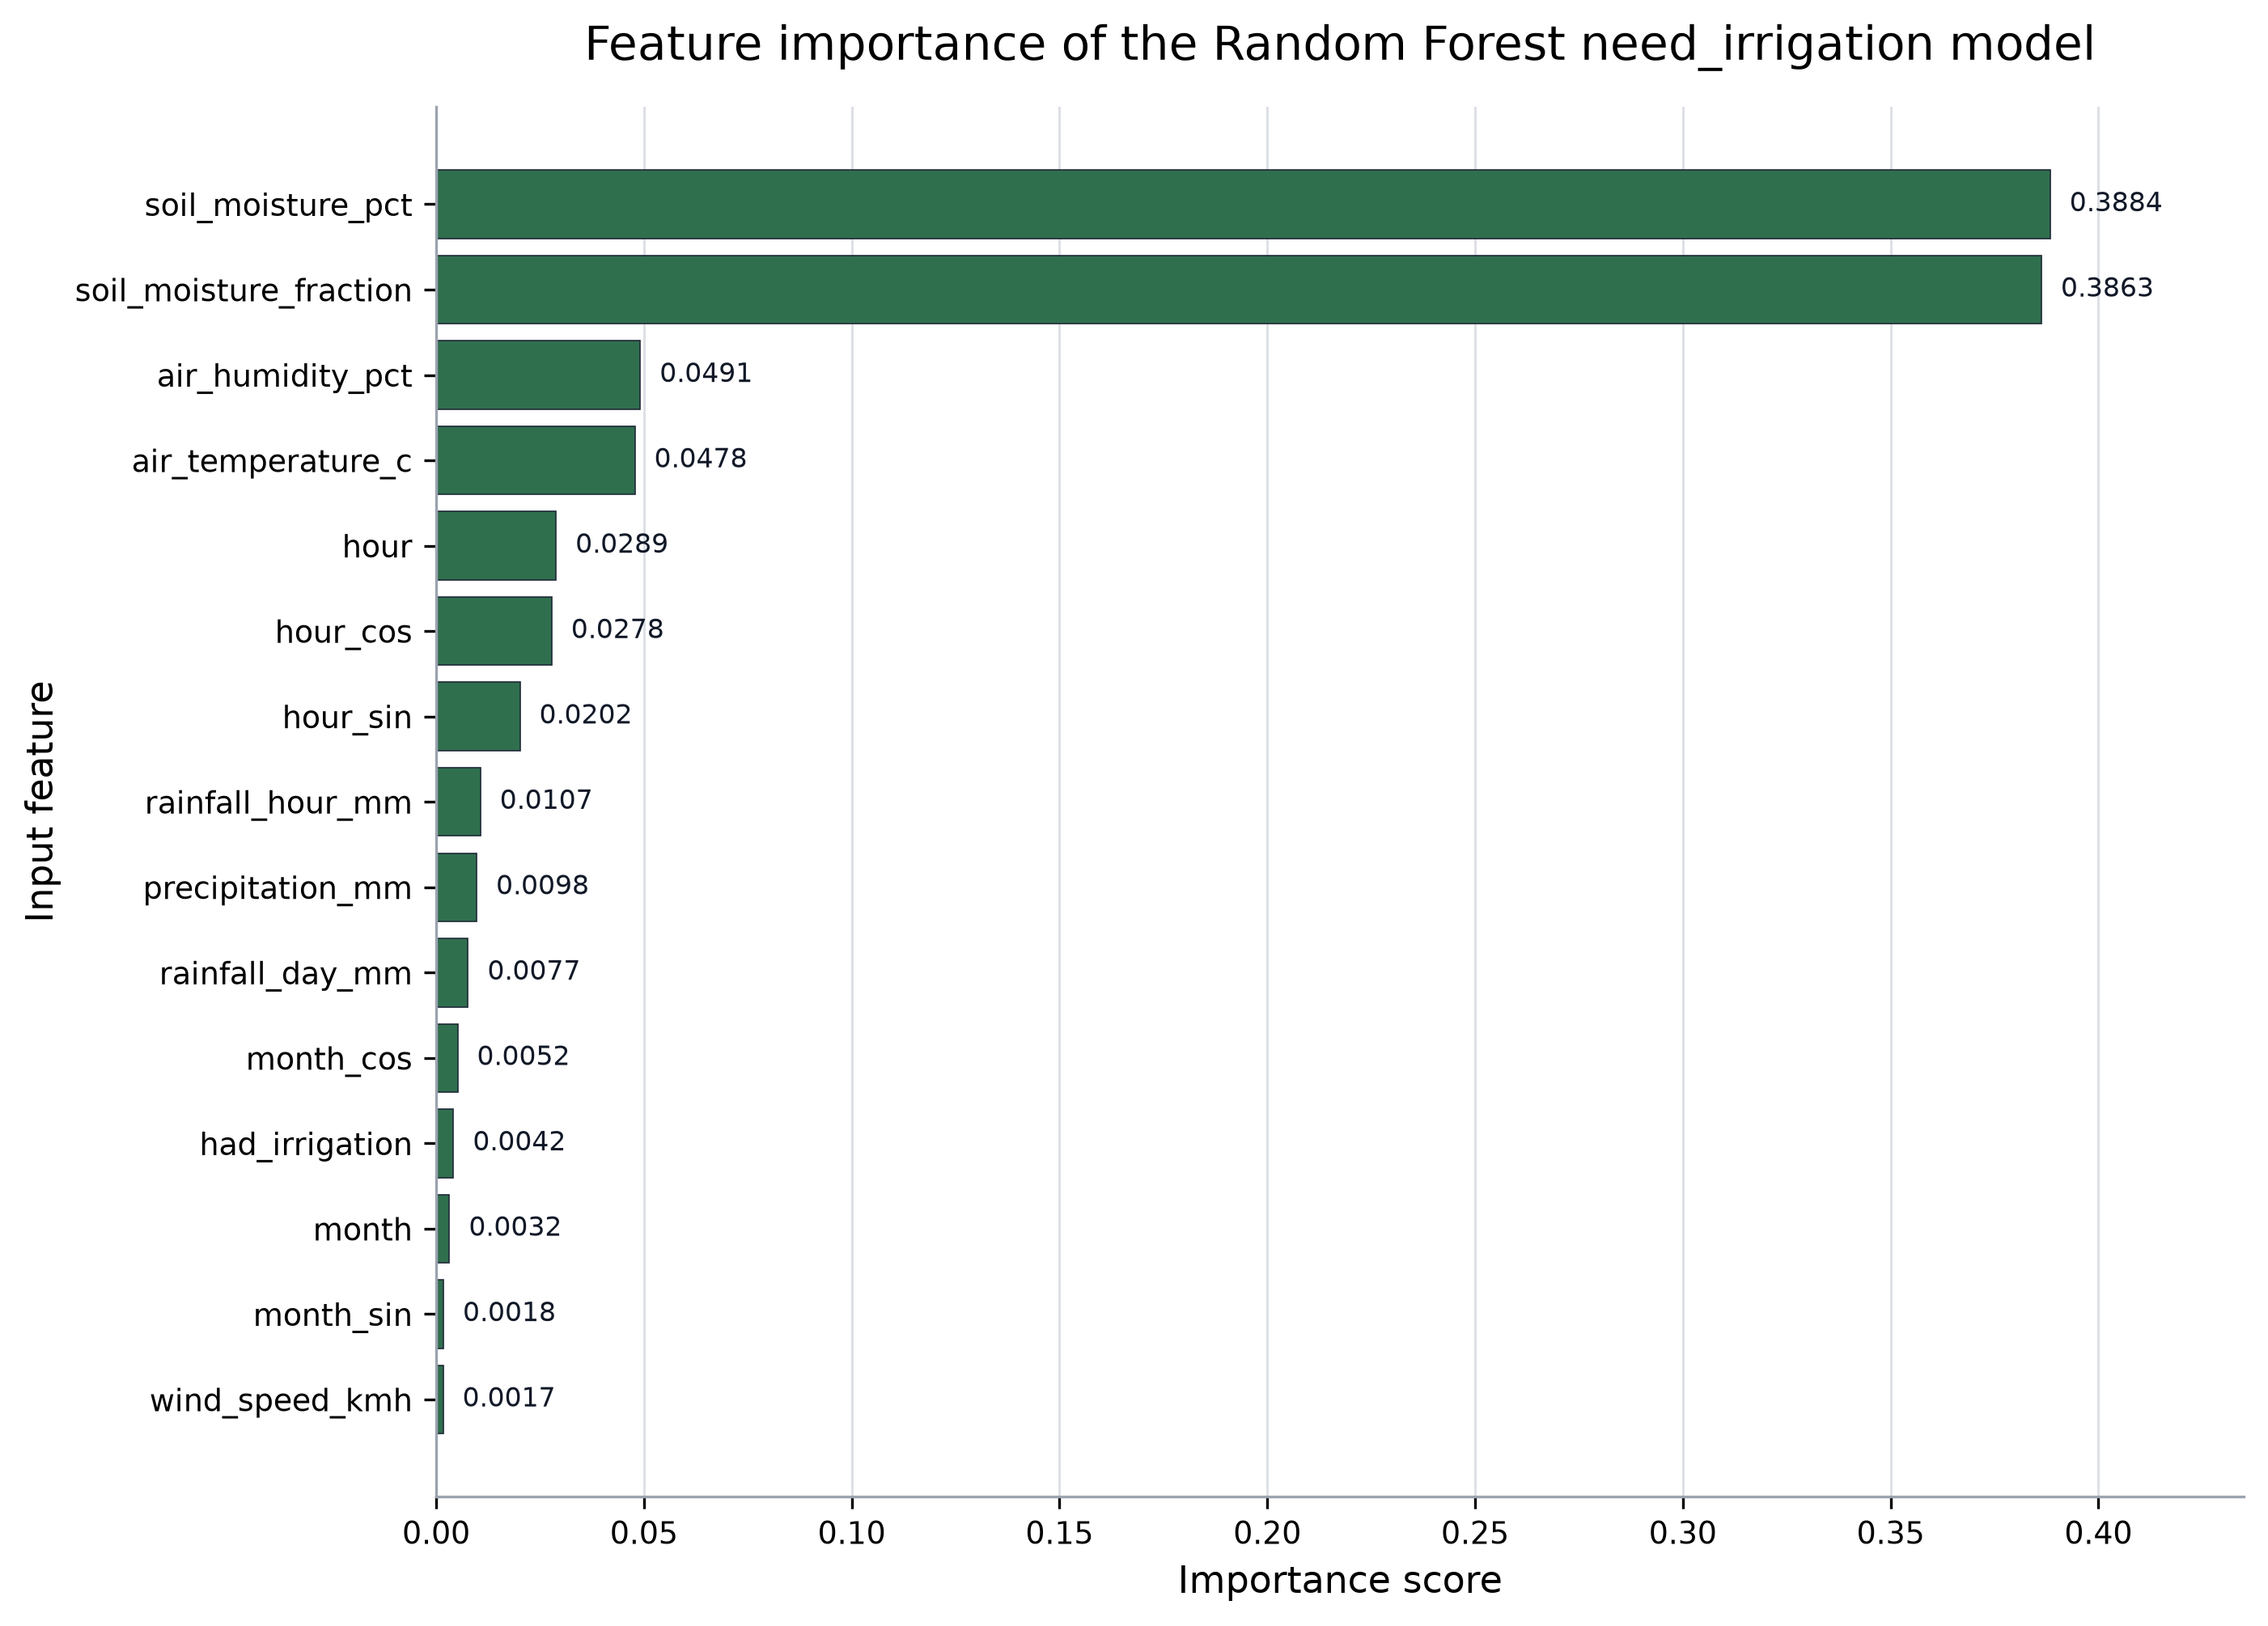
\includegraphics[width=0.9\textwidth,height=0.75\textheight,keepaspectratio]{figures/chapter_08/fig_8_7_need_irrigation_feature_importance.png}
    \caption{Feature importance of the Random Forest need\_irrigation model.}
    \label{fig:8-7a-feature-importance-of-the-random-forest-need-irrigation-model}
\end{figure}

\begin{figure}[H]
    \centering
    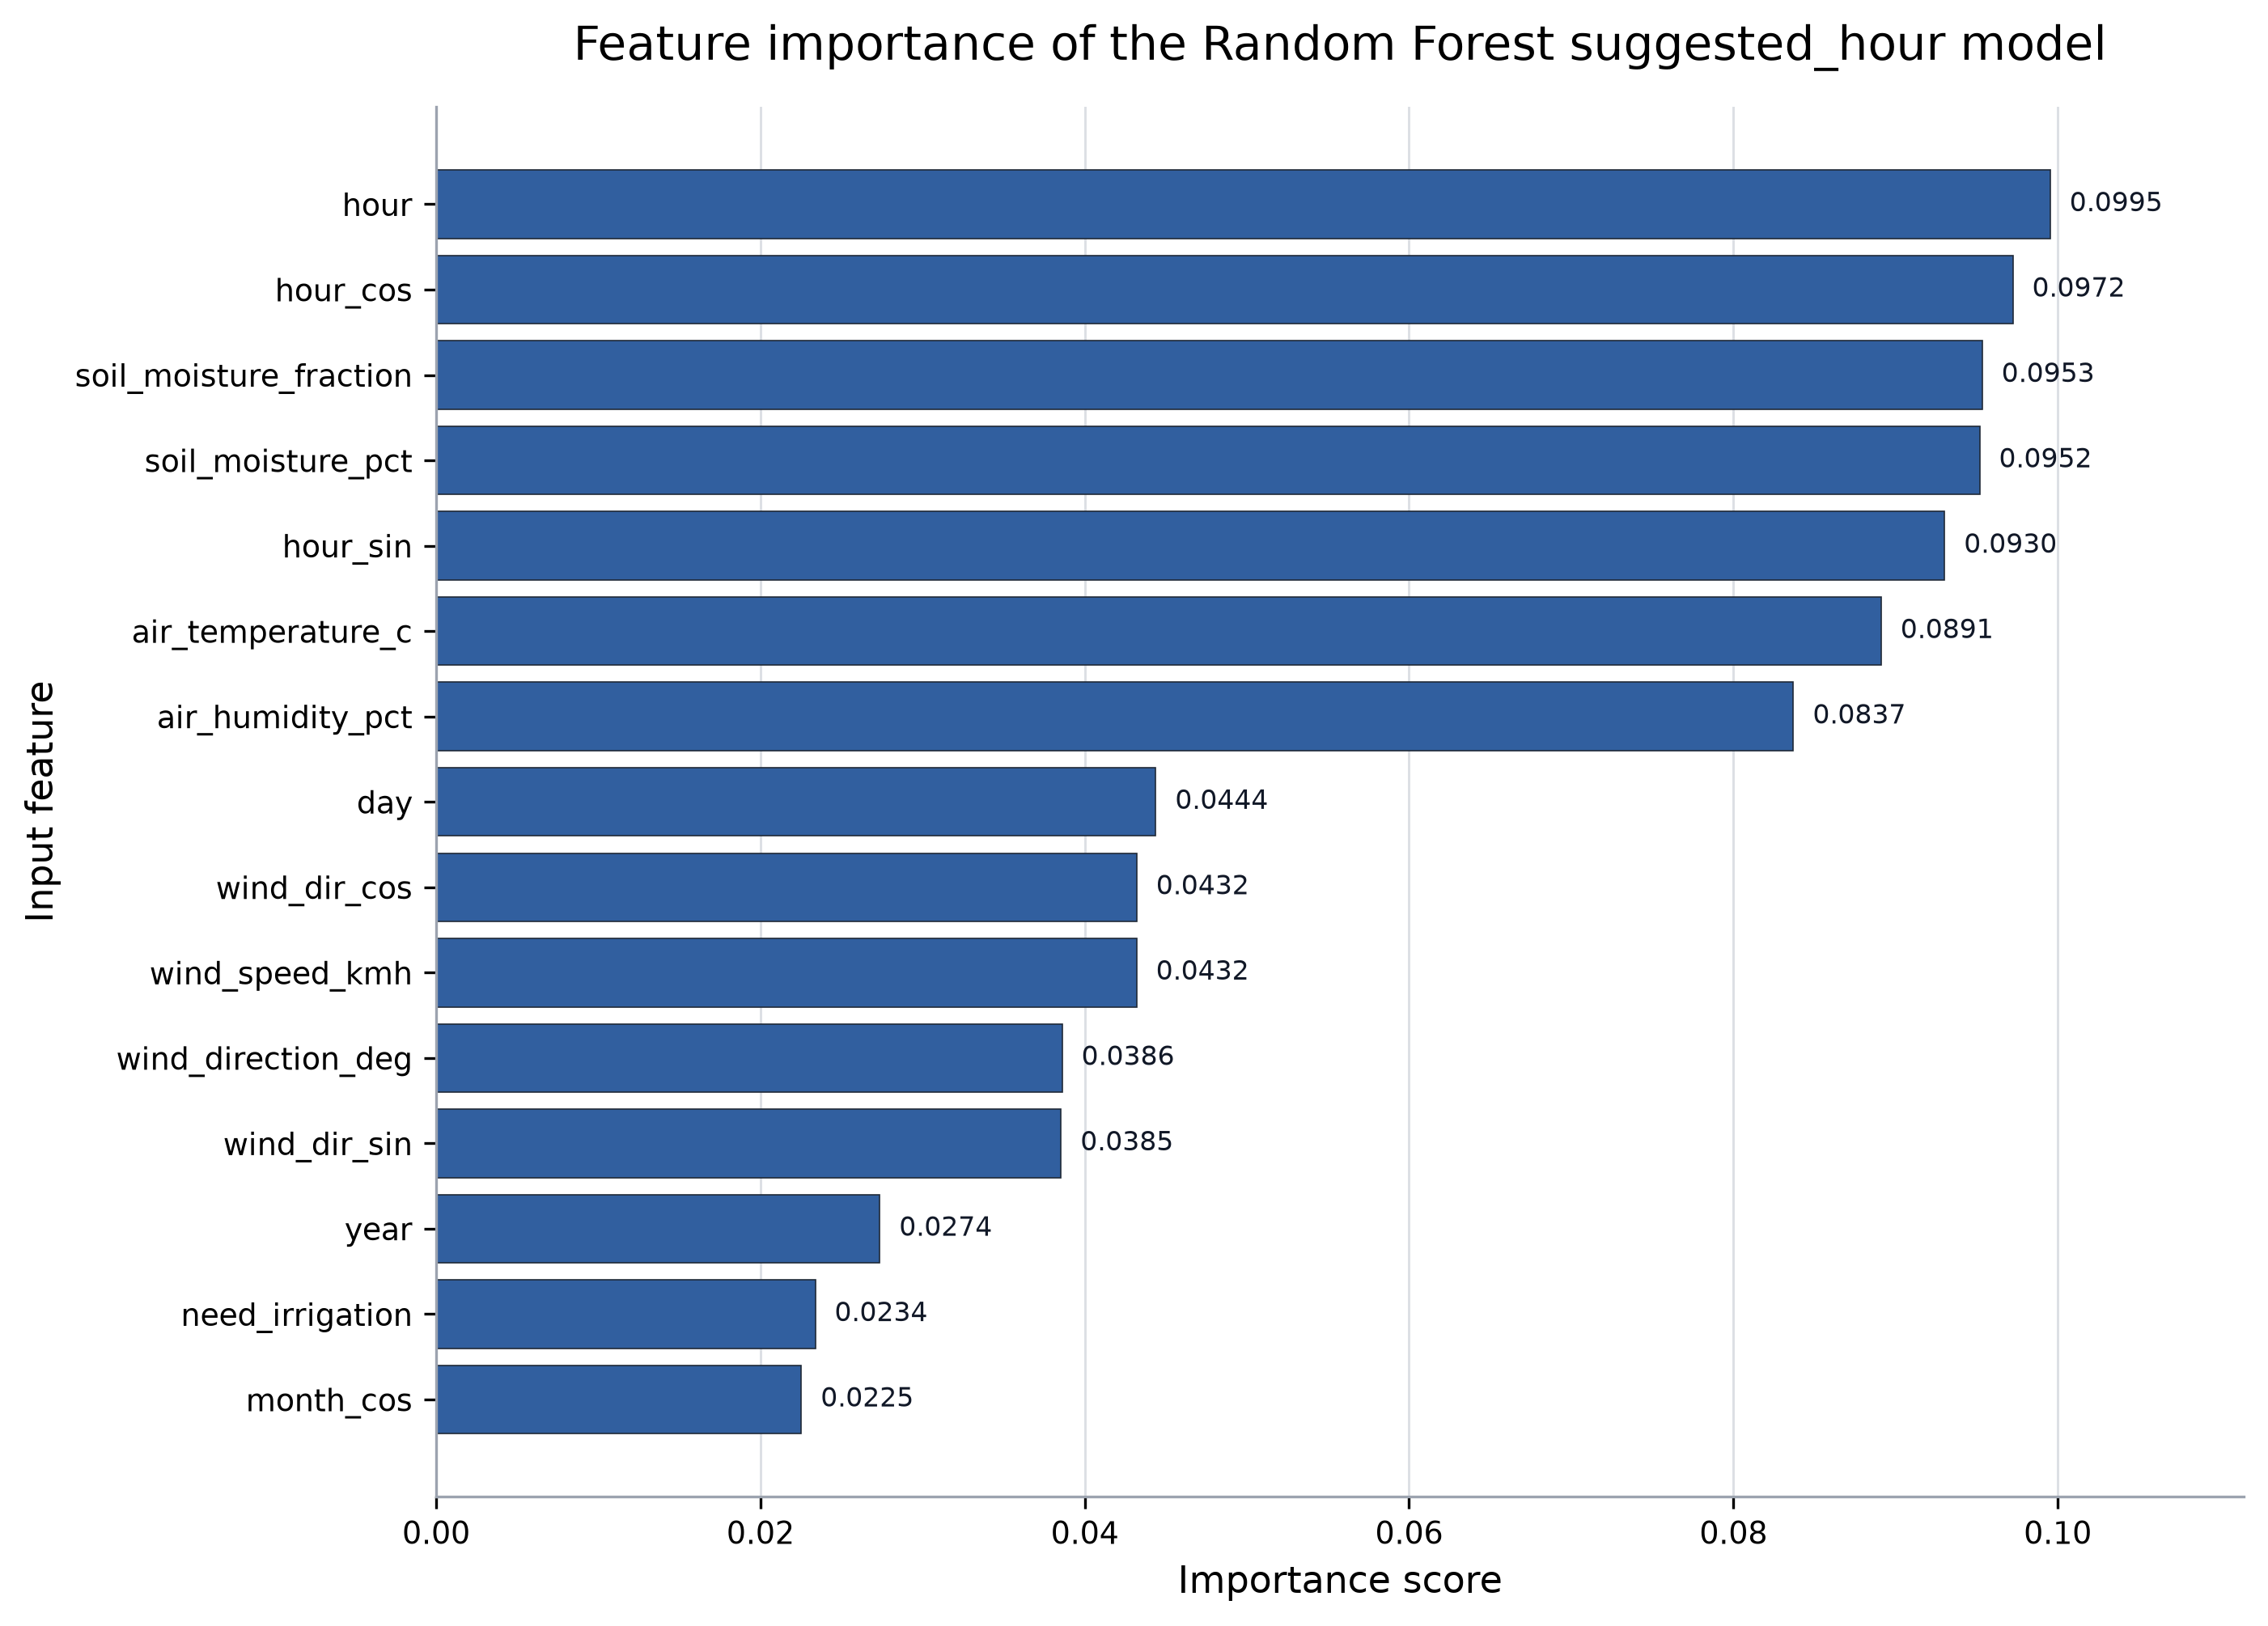
\includegraphics[width=0.9\textwidth,height=0.75\textheight,keepaspectratio]{figures/chapter_08/fig_8_8_suggested_hour_feature_importance.png}
    \caption{Feature importance of the Random Forest suggested\_hour model.}
    \label{fig:8-7b-feature-importance-of-the-random-forest-suggested-hour-model}
\end{figure}

\begin{figure}[H]
    \centering
    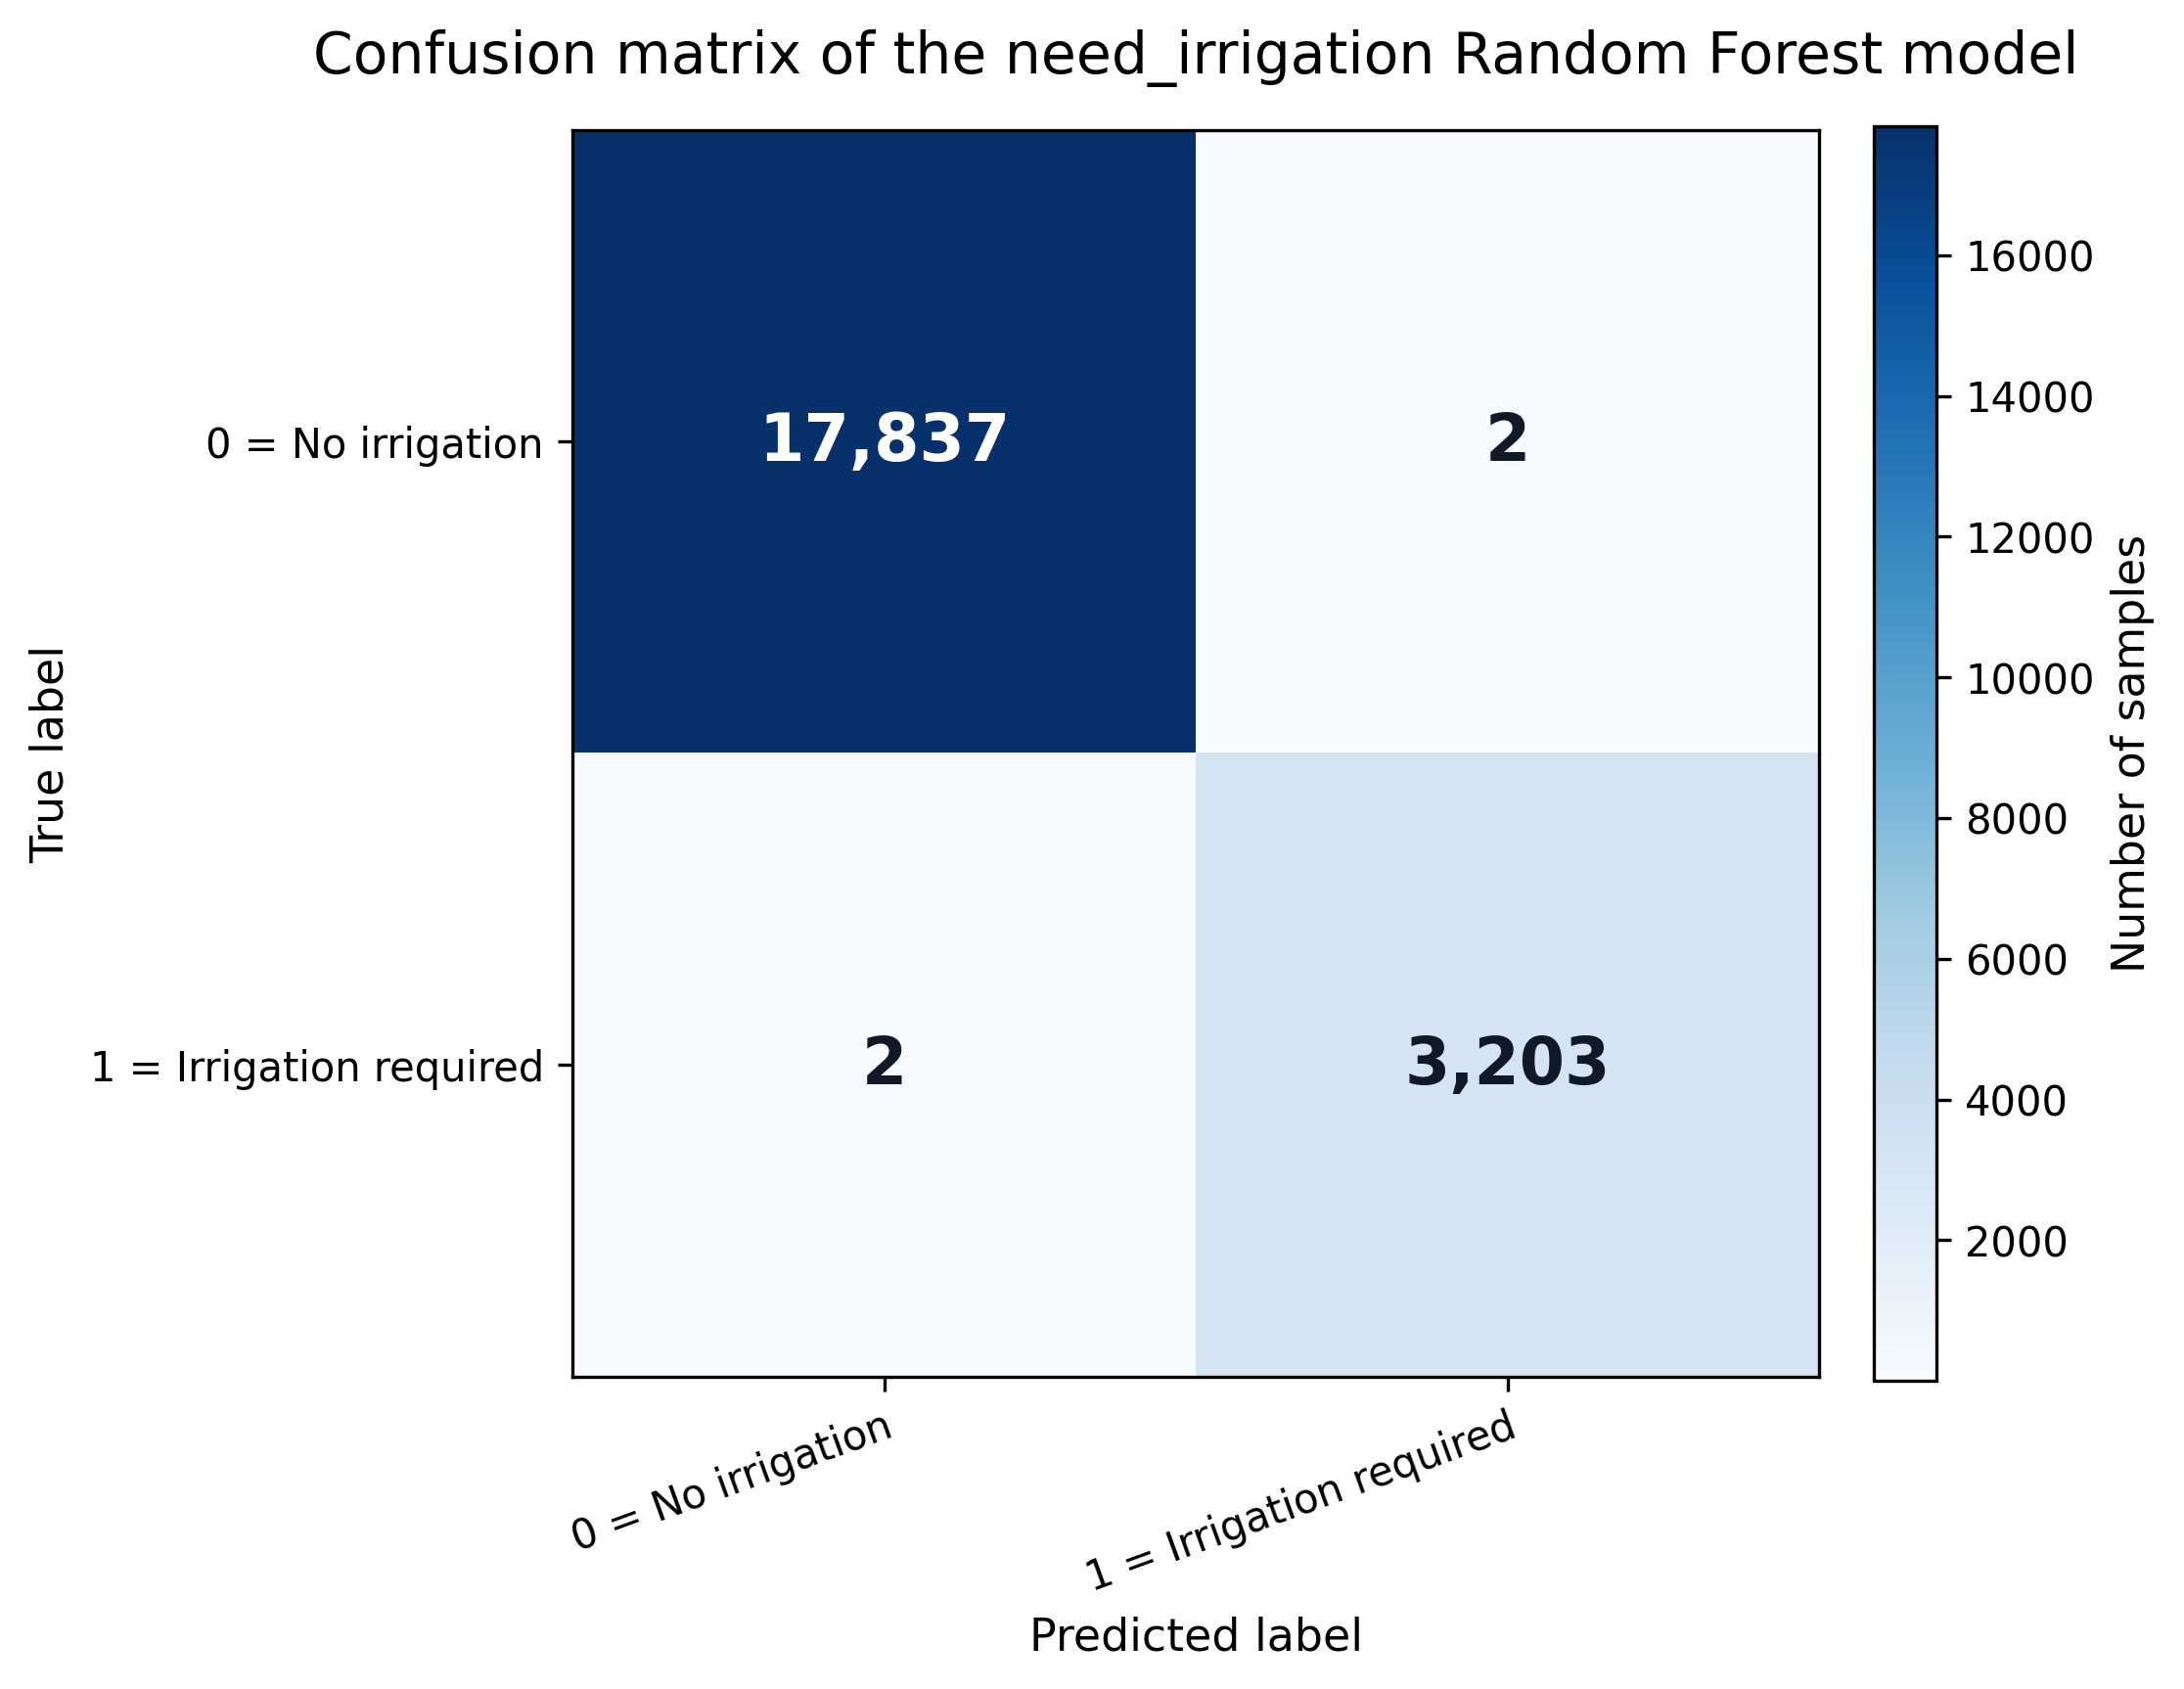
\includegraphics[width=0.9\textwidth,height=0.75\textheight,keepaspectratio]{figures/chapter_08/fig_8_9_need_irrigation_confusion_matrix.png}
    \caption{Confusion matrix of the need\_irrigation Random Forest model.}
    \label{fig:8-8a-confusion-matrix-of-the-need-irrigation-random-forest-model}
\end{figure}

\begin{figure}[H]
    \centering
    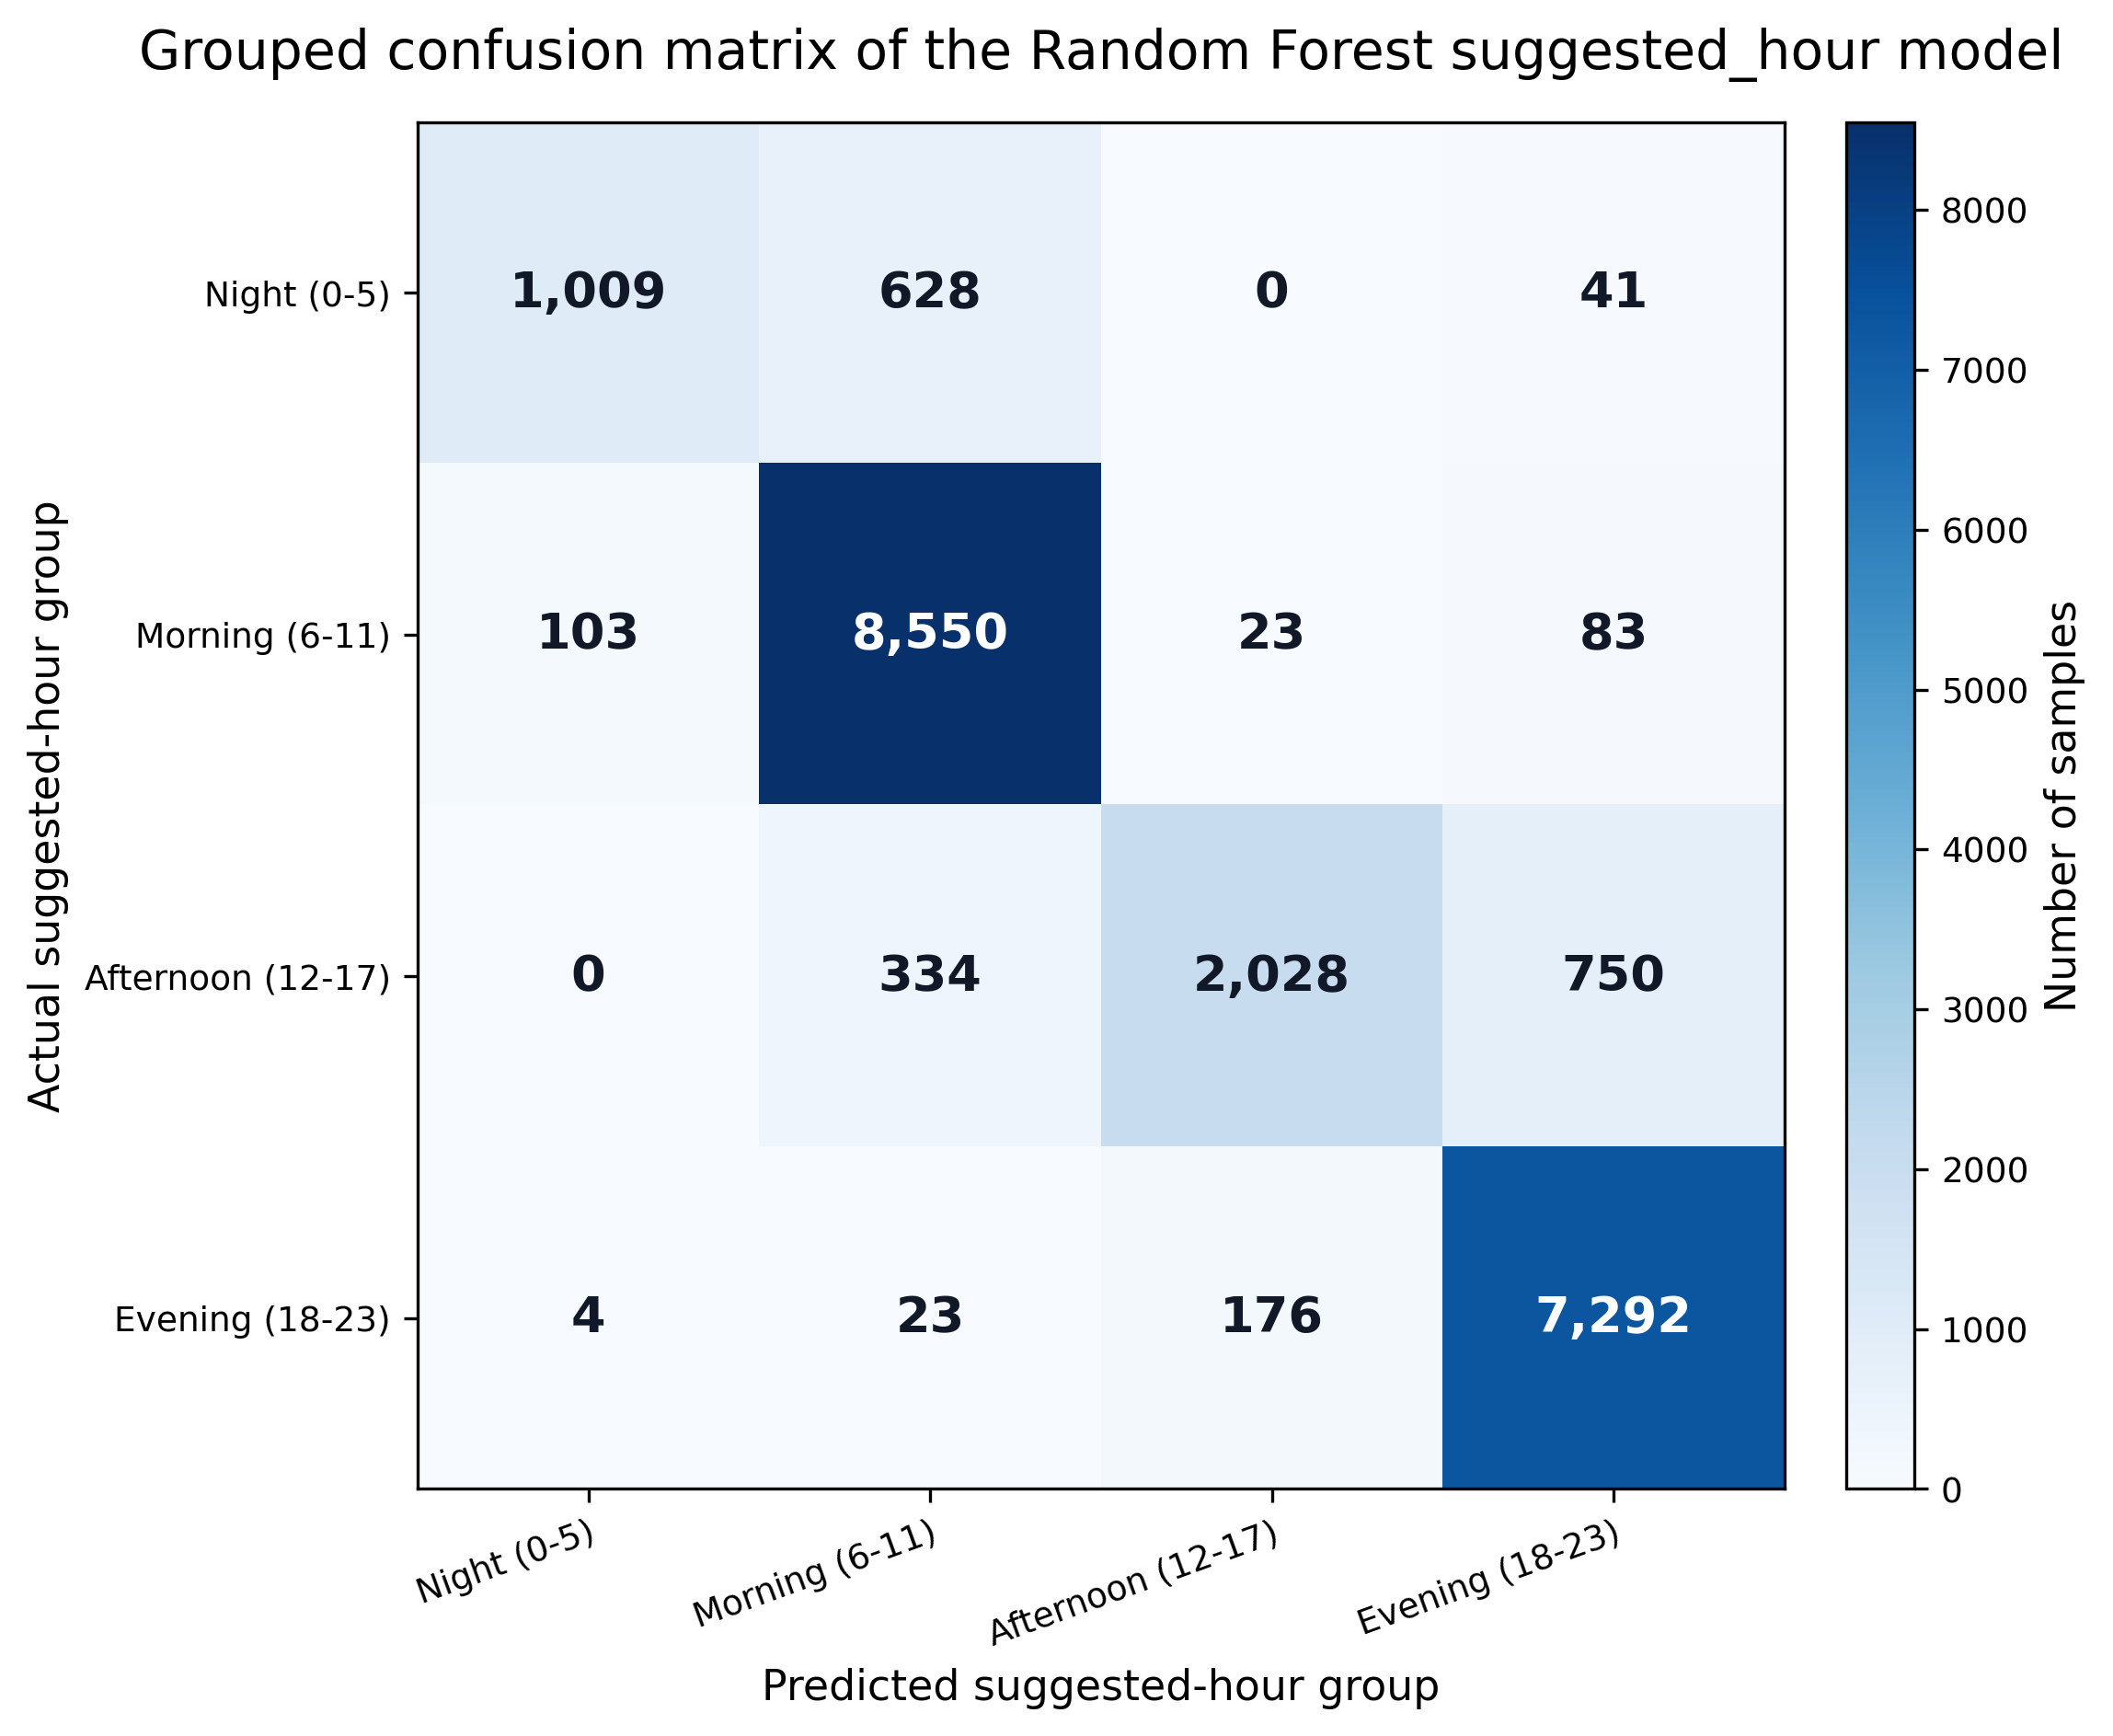
\includegraphics[width=0.9\textwidth,height=0.75\textheight,keepaspectratio]{figures/chapter_08/fig_8_10_suggested_hour_confusion_matrix_grouped.png}
    \caption{Confusion matrix of the suggested\_hour Random Forest model.}
    \label{fig:8-8b-confusion-matrix-of-the-suggested-hour-random-forest-model}
\end{figure}

\section{Limitations}

The ML layer is limited by the dataset used, the controlled prototype context, and the absence of long-term multi-crop field validation. Model results must therefore be interpreted cautiously. Future work should include retraining using real field data, comparing alternative models, and validating irrigation recommendations under real agronomic conditions.

\section{Conclusion}

This chapter described the intelligent layer of Agrio. It explained how the dataset is adapted for Random Forest training, how exported model artifacts are loaded by the ML service, how runtime prediction is connected to the Digital Twin state, and how simulation and recommendation functions transform measurements into irrigation support. The chapter also clarified the limits of the current validation: the ML results demonstrate reproducible dataset-level inference, while long-term agronomic validity still requires real field experiments.
